\documentclass[12pt,oneside]{fithesis}
%\documentclass[12pt,draft,oneside]{fithesis}
\usepackage[utf8]{inputenc}
\usepackage[IL2]{fontenc}
\usepackage[plainpages=false, pdfpagelabels]{hyperref}
\usepackage{paralist}
\usepackage{graphicx}
\usepackage{amsmath}
\usepackage{color}
\usepackage{courier}

\usepackage{minted}
%\usemintedstyle{bw}

%\usepackage{fontspec}
%\setsansfont{Calibri}
%\setmonofont{Consolas}

\usepackage{float}
\floatstyle{ruled}
\newfloat{program}{thp}{lop}
\floatname{program}{Listing}


\thesistitle{Design and implementation of a social network for making acquaintances}
\thesissubtitle{Bachelor thesis}
\thesisstudent{Marek Bryša}
\thesiswoman{false}
\thesisfaculty{fi}
\thesislang{en}
\thesisyear{spring 2012}
\thesisadvisor{doc. Ing. Michal Brandejs, CSc.}

\begin{document}
\FrontMatter
\ThesisTitlePage

\begin{ThesisDeclaration}
\DeclarationText
\AdvisorName
\end{ThesisDeclaration}

\begin{ThesisThanks}
Thanks
\end{ThesisThanks}

abstract

\MainMatter
\tableofcontents
\chapter*{Introduction}
\chapter{Design}
\section{Existing social networks for making acquaintances}
	\subsection{PlentyofFish}
		PlentyofFish (\url{http://www.plentyoffish.com/}) was founded in 2003 in Canada. It generates most of it's revenue through advertising and some premium services. Unfortunately, it currently only serves users from Canada, UK, US, Australia, Ireland, New Zealand, Spain, France, Italy and Germany, so the author could not sign up at all.
		
		From the publicly available information, it allows users to create a profile, search for others, message and chat with them. A \emph{Chemistry test} and some other methods of finding a match are offered, but without explaining precisely how they work. \cite{website:pof}
		\subsection{Match.com}
		Match.com (\url{http://www.match.com}) was launched in 1995 and is one of the oldest networks. It requires a paid subscription ranging from 34.90 EUR for one month  to 77.40 EUR for 6 months.
		
		After signing up, the user is asked to upload a profile photo and fill in a detailed questionnaire about his or her character, interests, activities, relationships and preferences. Based on this information, the system tries to find the best matching partner. The user can then add the match to his or her favourites, follow their profile and message them. There is a special option to \emph{wink} at them which can be used to quickly bring attention of the user and wait for their response to quickly assess their general interest without the need to send a message. \cite{website:match}
		
		\subsection{OkCupid}
		OkCupid (\url{http://www.okcupid.com}) started in 2004. It claims to be the fastest growing website for making acquaintances.
		%TODO use dating???\\
		It is ad-supported and the essential features are free to use. A paid subscription called \emph{A-list} is also available for 14.95 USD/month. It removes the ads, allows advaced searching, changing of user name etc.
		
		Matches can be found through search using general criteria or by filling out questionnaires. A user can also create a his own questions, set their importance and expected answers. When another user fills them in, the system calculates a match percentage. This process is probably unique to OkCupid. \cite{website:okcupid}
		\subsection{eHarmony}
		eHarmony (\url{http://www.eharmony.com}) is a paid service that was launched in 2000. It claims to have more than 33 million members. Subscriptions cost from 59.95 USD for a month  to 239.4 USD for 12 months. It is primarily focused on finding a partner for marriage.
		
		The service uses personality tests, mathematical matching and expert advice to find the best match. There are separate subsites targeted for specific social groups such as Asians, Christians, Jews, gays, lesbians etc. A new user has to fill in a very detailed questionnaire about his current status, personality and preferences.\cite{website:eharmony}
\section{User data protection}
	When using this kind of social networks, the user usually has to provide information about himself that is very sensitive, even intimate. Protection of this data is therefore a very serious concern.
	
	The data is very valuable beyond it's original intent to find the best match. It can be used for instance to precisely target advertisements, give offers to buy new products and so on. Hence it is essential that the user is made clear how the information he enters on a website is used or if it is disclosed to third parties.
	
	The user should also have the ability to choose what data is shared with other users. In the best case this control should be very fine, i.e. the user should not be forced to share information in blocks, should be able to deny specified users access to his profile or parts of his profile etc. There should also be a simple tool to preview one's profile in the way others can see it.
	
	If a user deletes any data on his profile, it should be physically deleted from all the servers as well, unless it is expressly stated otherwise (e.g. for backup purposes).
	
	Any changes to the privacy policy of a website should be only done with sufficient prior notice, and preferably be opt-in. In this context, the user must have the ability to simply download all his or her data in a package and delete the account.
	
	The language of the privacy policy should be as simple as possible, for every user to clearly understand it. Almost no one will read a lengthy legal text which can lead to unfortunate misunderstandings later.
	
	It goes almost without saying that the servers must be well protected from hacker attacks, especially when they contain this kind of sensitive data. A successful attack would not only harm the users, but probably mark the end for the website. Ideally there should be a regular security audit that the users can review.

\section{The idea}
	TODO:
	\cite{Finkel01012012}
	From the research of existing social networks for making acquaintances we can conclude the following points and issues:
	\begin{itemize}
		\item The target audience are single people from about 20 to 60 years old.
		\item Many require a paid subscription to access even the most basic functionality.
		\item All require new users to fill in a long, detailed and intimate questionnaire. This can discourage many users.
		\item Therefore all collect very sensitive user data that could be potentially misused.
		\item All offer a method to quickly find a matching partner, but then require an action from one of the users to make a first contact. Some users might have trouble finding courage to do so.
	\end{itemize}

	To solve most of these issues, the author has come up with this idea for the new social network:
	\begin{itemize}
		\item The users will provide only general information: e-mail address, gender, year of birth, approximate location (county level), interest in men or women and a single profile photo.
		\item Based on simple search criteria such as age range, relative location to them (i.e. same county, neighbouring counties), they will browse profile pictures of other users one by one and mark the ones they like.
		\item Only once two users match their 'like' mark, both will be notified, added to their contact lists and be able to engage in real-time chat. Then they can get to know each other and possibly arrange a meeting.
	\end{itemize}
	
	This way only very little information is gathered in the database, which brings the user data privacy problems to a minimum, and it is not necessary to fill in any lengthy questionnaires. Users need not be shy when marking people they like, because until the mark is matched, the other person will not know about it.
	
	However this also brings some new issues. Because the marking of others is essentially only based on their looks, the target audience is going to be reduced to users for whom it is an important criteria. That means mostly younger people seeking fun rather than a serious relationship.
\chapter{Implementation}

\section{Technologies}
%TODO HTML5
%http://www.okcupid.com/about/technology
	It is very important to choose the right technology for the implementation of a project. We need to find the most suitable web application framework and a data store, if one is not hard-wired into the framework. The author has devised the following criteria for the evaluation of available technologies:
	\begin{itemize}
		\item \textbf{Availability for commercial use free of charge}\\
			Because of budgetary constrains, the technology must be free for commercial use. The project may later generate revenue through the use advertising.
		\item \textbf{General suitability for the project}\\
			It must facilitate creation of a website. It is expected that there will be a lot of HTTP requests that will make only little chages to the database, e.g. marking of photos a user likes. The data model will be quite simple. There must be an easy way of making HTTP push\footnote{"HTTP server push (also known as HTTP streaming) is a mechanism for sending data from a web server to a web browser." \url{http://en.wikipedia.org/wiki/HTTP_push}, {2012-04-08}} communication to enable real-time chat. 
		\item \textbf{Performance, scalability and stability}\\
			Again due to the low bugdet, the software must utilize the hardware as efficiently as possible. The user base could potentially grow very rapidly. It is therefore essential that all the system can match the growth cost efficiently. The framework should have a good track record of runtime stability.
		\item \textbf{Ease of development and developer community size}\\
			It should be easy to implement the project and good documentation is welcome. The framework should have a good community with which a developer can try to solve issues.
		\item \textbf{Codebase stability}\\
			The technologies should be past their rapid development phases and the core APIs should be stable. This minimizes the effort needed to transition the project to a newer version of the framework. 
		\item \textbf{Innovation factor}\\
			Younger technologies are preffered as their use can lead to innovation and discovery of new approaches to problems.
	\end{itemize}
	Because of the first criterion, our interest shall only be in open source frameworks.
	\subsection{General suitability for the project}
		The author is skilled in JavaScript, PHP, Python and Ruby, so we will further examine frameworks based on those languages. All have been used for HTTP server programming for a long time, except for JavaScript, which has emerged in recent years in the Node.js platform.\\
		\begin{table}[htb]
		\begin{tabular}{|r||p{2.2cm}|p{2.2cm}|p{2.1cm}|p{2.2cm}|}
			\hline 
			\rule[-1ex]{0pt}{2.5ex} & Node.js & PHP & Python & Ruby \\ 
			\hline\hline
			\rule[-1ex]{0pt}{2.5ex} Simple & Express.js & plain PHP & CherryPy & Sinatra \\ 
			\hline 
			\rule[-1ex]{0pt}{2.5ex} Full MVC & Locomotive, Railway.js & Zend, CakePHP & Dajngo, web2py & Ruby on Rails \\ 
			\hline 
		\end{tabular}
		\caption{Classification of web frameworks}
		\label{table:wf}
		\end{table}
	
		Table \ref{table:wf} shows a basic classification of selected web frameworks by programming language and complexity of features they provide. Simple frameworks generally only provide a way to route HTTP requests to methods, parse HTTP headers and to send a response. Other features can be added on using plugins or modules. Full MVC\footnote{Model-View-Controller} frameworks also have an ORM\footnote{Object-Relational Mapping} engine for models and generate HTML views using a templating engine.
		
		Because the project's uncomplicated data model would not utilize the complex feature set of full MVC frameworks and those could limit flexibility, we will further only focus on the simple ones, i.e. Express.js, plain PHP, CherryPy and Sinatra.
		
	\subsection{Performance, scalability and stability}
		Let us first compare performance of the languages and their virtual machines themselves. We can use results from \emph{The Computer Language Benchmarks Game} \cite{website:bench}. It uses several algorithms written in different programming languages to measure their speed.
		
		\begin{figure}[htb]
	  \centering
	    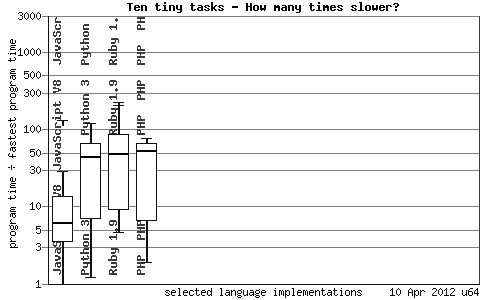
\includegraphics[width=0.7\textwidth]{bench2.png}
		  \caption{Language benchmark of V8 Engine, Python 3, Ruby 1.9 and PHP 5.4.0. Lower means faster. Source: \cite{website:bench}}
		  \label{fig:bench1}
		\end{figure}
		
		A box plot of the benchmark is shown in figure \ref{fig:bench1}. The vertical axis means how many times the language is slower than the fastest one (Intel Fortran 12.1). Out of the languages under consideration, Node.js on average 6 times faster than the rest\footnote{Node.js uses the V8 Engine internally}. 
		
		Next we will benchmark the performance of the HTTP handling of the frameworks. All the tests will be run on a dual-core i686 Linux 3.2.11 PC with 4GB of RAM. We will use the Apache HTTP server benchmarking tool (\texttt{ab}). Source codes for Sinatra and Node.js are in listings \ref{code:sinatra} and \ref{code:nodejs}, the other two for PHP and CherryPy are on the attached CD.

		\begin{program}
		\caption{Benchmark for Sinatra in Ruby}
		\label{code:sinatra}
		\inputminted[fontsize=\footnotesize]{ruby}{../bench/sinatra/app.rb} 
		\end{program}
		
		\begin{program}
		\caption{Benchmark for Node.js in JavaScript}
		\label{code:nodejs}
		\inputminted[fontsize=\footnotesize]{javascript}{../bench/nodejs/app.js}
		\end{program}

		The \texttt{add} method has two parameters \texttt{a} and \texttt{b} and simply returns their sum. It will simulate simple \texttt{GET} parameter parsing and response.
		
		The \texttt{sleep} method has one paramater \texttt{ms}. Execution is suspended for \texttt{ms} miliseconds and a simple response is sent. This is intended to simulate a database query that takes given time. We will use a 20ms delay.
		
		Node.js uses its internal HTTP server, Sinatra uses the Thin server, CherryPy uses its internal WSGI server and PHP is hosted through \texttt{mod\_php} on the Apache server. Unlinke CherryPy and Apache which use a thread pool to serve requests, Node.js and Thin use the \texttt{libevent} that utilizes \texttt{epoll} on Linux and \texttt{kqueue} on FreeBDS theoretically allowing for better concurrency. Node.js is also strictly single-threaded.
	
		Here is a list of versions and parameters used:
		\begin{compactitem}
			\item Node.js 0.6.13
			\item PHP 5.3.10, Apache 2.2.22
			\item Python 3.2.2, CherryPy 3.2.2, 100 threads in the pool
			\item Ruby 1.9.3p125, Sinatra 1.2.7, Thin 1.3.3
			\item All logging including access is disabled.
			\item 5000 request per test
			\item Concurrency in set (1,10,30,50,100,200,300,500,700,1000)
			\item \texttt{ab} is run 10 times for each parameter set and a mean is calculated.
			\item \texttt{/proc/sys/net/ipv4/tcp\_tw\_reuse} set to 1. This allows for reuse of sockets in the \texttt{TIME\_WAIT} state. This is a recommanded setting for high concurrency web servers. 
			\item 2 seconds wait time between each run of \texttt{ab}
			\item In case one of the runs fails (i.e. any of the 5000 requests fails), a score of 0 request per second is awarded for the run.
			\item Source code of the Python script used to perform the benchmark can be found in attached file \texttt{bench.py}.
		\end{compactitem}
		
		Graph \ref{fig:bench_add} shows the results of the \texttt{add} benchmark. We can see that PHP keeps up with Node.js until the 100 concurrent requests mark, but then declines sharply. Node.js is able to serve about 4700 request per second regardless of concurrency.
		
		Graph \ref{fig:bench_sleep} shows the results of the \texttt{sleep} benchmark. Node.js is again the clear winner with about 4700 request per second regardless of concurrency. This is because Node.js's \texttt{setTimeout} is non-blocking. This applies also to any database query. Once the query is made, Node.js moves to serve other requests.
		
		\begin{figure}[h]
	  \centering
	    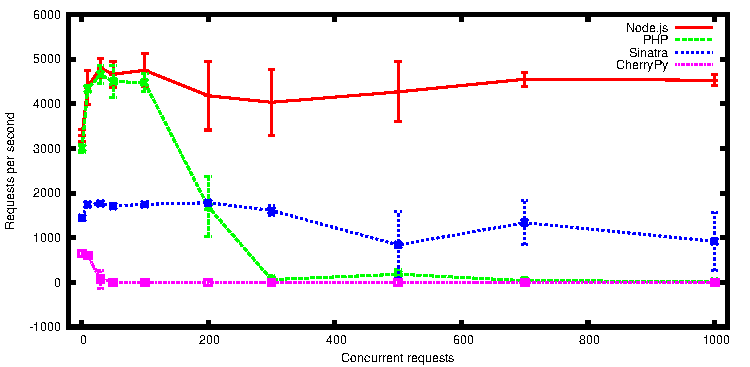
\includegraphics[width=1.0\textwidth]{plot_add.pdf}
		  \caption{Benchmark of the \texttt{add} method. Error bars denote standard deviation.}
		  \label{fig:bench_add}
		\end{figure}		
		\begin{figure}[h]
	  \centering
	    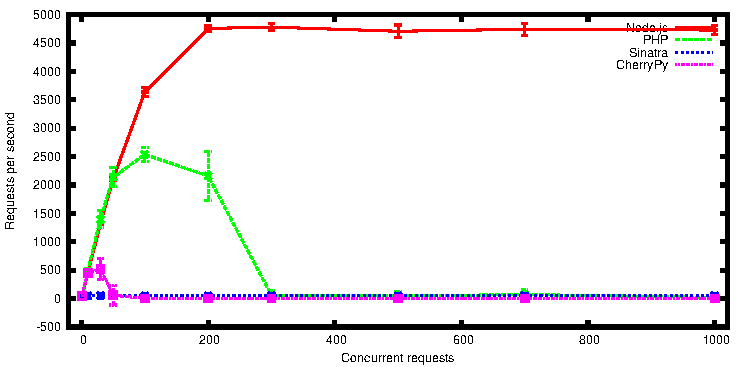
\includegraphics[width=1.0\textwidth]{plot_sleep.pdf}
		  \caption{Benchmark of the \texttt{sleep} method. Error bars denote standard deviation.}
		  \label{fig:bench_sleep}
		\end{figure}
		
		Node.js and Sinatra on Thin are the only framework to remain stable with increasing load. PHP and CherryPy have started dropping requests at concurrency levels of 300 and 30 respectively.
				
		In conclusion, Node.js performs the best as both a language and a HTTP server framework and remains stable under any load. Sinatra is also stable, however it is slower, which could be partially solved by the use of clustering. Under low loads PHP on Apache is just as fast as Node.js, but it's stability is hardly acceptable. CherryPy is eliminated.
		
	\subsection{Ease of development and developer community size}
		All the frameworks in the comparison provide very similar levels of functionality. From the author's experience, Ruby allows for shortest code at the slight expense of readability. Javascript on the other hand requires the longest code and can be a little tricky. See aganin listings \ref{code:sinatra} and \ref{code:nodejs}.
		
		PHP is arguably the most used framework for web programming, hence it has the biggest developer community. It is well documented in many languages. Countless modules, snippets and add-on libraries are available.
		
		Node.js and Sinatra have a smaller but very active community. Thousands of modules and add-on are available through their package managers such as npm for Node.js and RubyGems for Sinatra. Both are adequately documented if not deeply. 
		
	\subsection{Codebase stability}
		PHP's codebase is the most stable. It is the oldest framework in the comparison, laguage and API changes are almost non-existen and don't break backwards compatibility.
		
		Sinatra and Node.js split the second place. There have still been some changes to the Ruby language from version 1.8 to 1.9 that could break backwards compatibility. Node.js is still under active development, however the API tends to only grow and not change.
		
	\subsection{Innovation factor}
		Node.js is the clear winner in this criterion. It is the most innovative in that it uses JavaScript on the server side, event-based polling and non-blocking API.
		
		Sinatra comes in the second place. It utilizes Ruby's advanced language constructions allowing for tidy coding. PHP finishes last because of its age and lack of modern approaches.
		
	\subsection{The overall winner: Node.js}
		The author has chosen Node.js for the implementation of this project. It is just as suitable as other frameworks and clearly wins performance, scalability and stability tests. It is also the most innovative framework of recent years with growing developer community support.
		
		There are two drawback to using Node.js. Firstly it is still relatively immature and bigger API chages could still happen. Secondly the use of JavaScript and non-blocking function calls can lead to poorly readable code. The author however believes that the advantages greatly outweigh this.
	\subsection{Data store}		
		The decision to use simple web framework gives us a free hand in choosing a separate data store. The traditional choice is an SQL database, e.g. MySQL and PostgreSQL. Lately NoSQL databases (MongoDB, CouchDB etc.) and  advanced key-value storages such as Redis have come into focus. In a recent paper \emph{Social-data storage-systems} \cite{Ruflin2011} that compares all of above, no clear winner is given.
		
		The author has chosen Redis. "Redis is an open source, advanced key-value store. It is often referred to as a data structure server since keys can contain strings, hashes, lists, sets and sorted sets."\cite{website:redis} Redis keeps the entire database in memory with optional regular persistent storage snapshots, which allows for very fast read/write access and good reliability.	Benchmarks such as \cite{website:ruturaj} show that Redis is about eight times af fast as MySQL when it comes to simple operations.
		
		One of the drawbacks is that Redis mostly has simple commands so even moderately complex operations are difficult to program.
		
		The innovation factor is high because Redis is usually not used as a single storage for all the data. As a bonus, Redis contains a simple publisher-subscriber functionality, which will come handy when implementing the real-time chat.
	\subsection{Modules and libraries used}
		The following libraries and modules will be used to simplify implementation of the project:
		\begin{itemize}
			\item[\textbf{Underscore.js}] "A utility-belt library for JavaScript that provides a lot of the functional programming support that you would expect in Prototype.js (or Ruby), but without extending any of the built-in JavaScript objects." \footnote{\url{http://documentcloud.github.com/underscore/} 2012-04-18} It will be used in both client and server JavaScript code. 
			\item[\textbf{Express.js}] A simple web framework on top of Node.js. Allows for easy routing, GET and POST method parameter parsing and response sending. Uses the common \texttt{Connect} architecture, therefore  is also a base for other modules.  \url{http://expressjs.com/}
			\item[\textbf{node-jade}] A library for the Jade HTML templating engine. \url{http://jade-lang.com/}
			\item[\textbf{redis}] A Node.js Redis client. Performance can be enhanced using the \texttt{hiredis} native backend. \url{https://github.com/visionmedia/connect-redis}
			\item[\textbf{connect-redis}] A \texttt{Connect} module for saving of user session data to the Redis data store. Uses a signed cookie for client identification. \url{https://github.com/visionmedia/connect-redis}
			\item[\textbf{node-sechash}] A library for calculation of cryptographically secure hashes to be used to store passwords. Automatically adds salt. \url{https://github.com/kbjr/node-sechash}
			\item[\textbf{formaline}] An advanced HTTP POST request parser. Especially useful to handle file uploads. \url{https://github.com/rootslab/formaline}
			\item[\textbf{node-gm}] A Node.js GraphicsMagick library. Facilitates image manipulation such as resizing, cropping and format coversion. \url{http://aheckmann.github.com/gm/}
			\item[\textbf{i18n-node}] A simple internationalization library. \url{https://github.com/mashpie/i18n-node}
			\item[\textbf{async}] A library to simplify asynchronous function calls on arrays of data, typically in series or parallely. \url{https://github.com/caolan/async}
			\item[\textbf{RedBack}] "A fast, high-level Redis library for Node.JS that exposes an accessible and extensible interface to the Redis data types." \footnote{\url{http://redbackjs.com/} 2012-04-18} Its \texttt{RateLimit} class will be used for spam protection. 
			\item[\textbf{node-recaptcha}] A Node.js reCaptcha service client. Used for spam prevention. \url{https://github.com/mirhampt/node-recaptcha}
			\item[\textbf{socket.io}] WebSocket and HTTP push library. \url{http://socket.io/}
			\item[\textbf{node-amazon-ses}] A Node.js module for sending e-mail using the Amazon SES cloud service. \url{https://github.com/jjenkins/node-amazon-ses}
			\item[\textbf{cluster}] A Node.js module for managment of multiple server instances. \url{https://github.com/LearnBoost/cluster}
			\item[\textbf{jQuery}] HTML DOM and CSS manipulation library for JavaScript. \url{http://jquery.com/}
			\item[\textbf{jquery.validate}] jQuery plugin for HTML form validation. \url{http://bassistance.de/jquery-plugins/jquery-plugin-validation/}
			\item[\textbf{jquery.Jcrop}] jQuery plugin for image cropping. \url{http://deepliquid.com/content/Jcrop.html}
			\item[\textbf{jquery.elastic}] jQuery plugin that grows textareas automatically. \url{http://unwrongest.com/projects/elastic/}
			\item[\textbf{UglifyJS}] A JavaScript minifier and obsfucator. \url{https://github.com/mishoo/UglifyJS}
		\end{itemize}
\section{Data model}
	Redis is a key-value storage, therefore there is no fixed schema for the database and no hierarchy per se.  As a convention, a colon character is used to divide key names into logical subgroups, e.g. \texttt{user:1234:email}. 
	
	A complete plan of the structure of the database is included in appendix \ref{appendix:scheme}.
	\subsection{Redis work-flow}
	Simple user parameters are stored as a Redis hash in order to reduce the total number of top-level keys, which can have an impact on the performance. For example to access the e-mail address of user with \texttt{id} 1234, one has to issue Redis command \mint{text}|HGET user:1234 email| insted of \mint{text}|GET user:1234:email|
	
	
	An introduction to the data types and basic commands of Redis is available at \url{http://redis.io/topics/data-types}.
	
	There is a way to search all key names for a given pattern using the \texttt{KEYS} command, but it is very slow compared to other commands. Therefore to keep track of the objects it the database, a set of their ids must be kept. For instance to create a new user one has to execute the sequence from listing \ref{code:ex-user}.
	
	First a user id is generated by increasing the counter. Then a \texttt{multi} command is started. This guarantees that everything will be process at once. Since Redis is single-threaded, it is atomic by default.
	
	Also note the use of asynchronous function calls --- one of the defining characteristics of Node.js.
	\begin{program}[h!]
	\caption{An excerpt of user creation code}
	\label{code:ex-user}
	\inputminted[fontsize=\footnotesize, linenos=false]{javascript}{ex-user.js}
	\end{program}
	
	
\section{Basic functionality}
	\subsection{User registration}	
	  \begin{figure}[h]
	  \centering
	    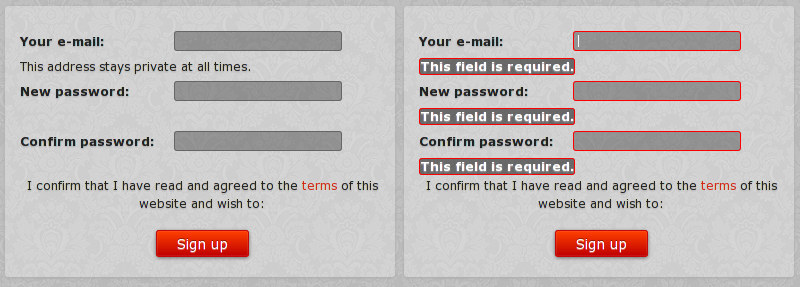
\includegraphics[width=1.0\textwidth]{screen-signup.png}
		  \caption{Sign up form.}
		  \label{fig:screen-signup}
	  \end{figure}
		The user is presented with a registration form on the homepage. There are three fields: e-mail address, password and password confirmation. The e-mail field uses the HTML5 \texttt{email} type, which causes supporting browsers to simplify input, for instance by displaying the \texttt{@} character on a virtual keyboard on touch input devices. A minimum of 6 characters is required for the password. When the user clicks the Sign up button, the values are validated with the jquery.validate plugin and errors are highlighted, see figure \ref{fig:screen-signup}. The pluing prevents the form from being submitted with errors.
		
		If there have been more than three registrations from a given IP address within the last 12 hours, a reCaptcha is displayed to prevent automated malicious user registrations. The \texttt{RateLimit} class of the RedBack module is used to efficiently store the number of registrations.
		
		When the form is posted to \texttt{/signup}, all values and the reCaptcha are once again validated on the server side. This is indeed necessary, since it is very easy to circumvent any client side validation. User attributes are added to the database. The password is stored using the \texttt{sechash}, which makes it more diffucult to get users' passwords even if the database is hacked.
		
		An e-mail is sent to the user's address, containing a welcome message and a verification code, see section \ref{section:email}. Then the user is redirected to the second phase of the registration.
		
		\begin{figure}[h]
	  \centering
	    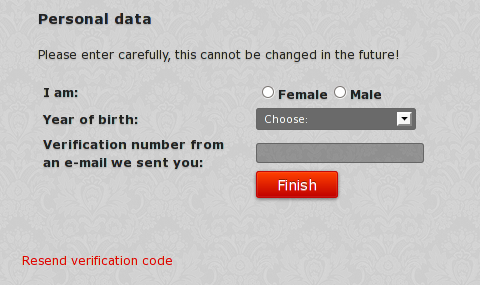
\includegraphics[width=0.7\textwidth]{screen-signup1.png}
		  \caption{Second phase of signup.}
		  \label{fig:screen-signup1}
	  \end{figure}
	  There the user is asked to enter his or her gender, year of birth and the verification code. It is a random number in the range $\left[ 100,999\right)$. This is intended to make it simple for the user to remember it for the few seconds while switching windows. On the other hand would also make it simple to quickly guess the right one, circumventing the e-mail verification. There is however a hard limit of 3 wrong attempts. An option to resend the verification code is also given, with a limit of 3 per 12 hours.
	  
		\begin{figure}[h]
	  \centering
	    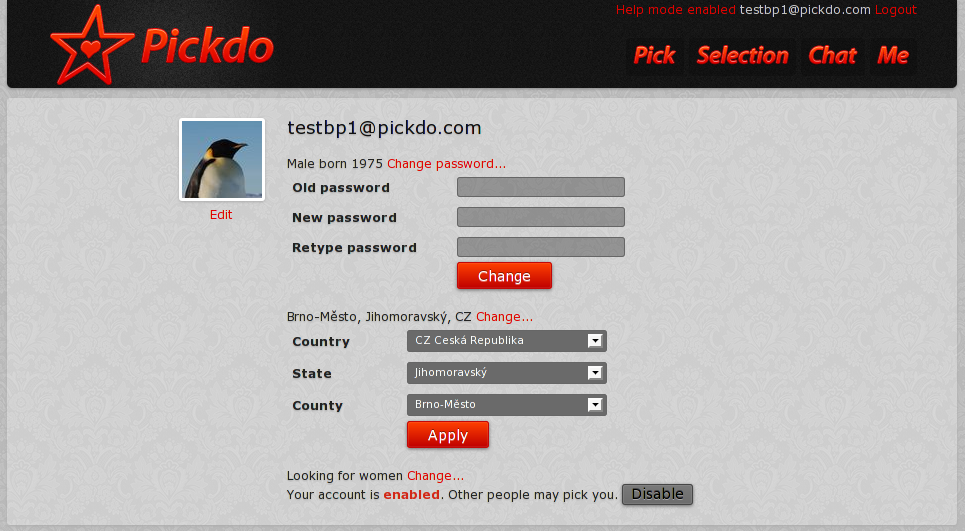
\includegraphics[width=0.9\textwidth]{screen-profile.png}
		  \caption{Profile and settigs page. (Author of the penguin photo: Hannes Grobe/AWI, CC-BY-SA 3.0)}
		  \label{fig:screen-profile}
	  \end{figure}	  
	  
	  After that, the user is redirected to his or her profile page, where his or her approximate location must be entered and a profile photo uploaded in order to fully enable the account (see figure \ref{fig:screen-profile}). More on geolocation in section \ref{section:geo}.
	  
	  Users have the ability to disable their accounts for the case they have found their acquaintance or are no longer looking for one. This causes notifications for their account to stop and they are no longer able to search for new users.
	\subsection{Photo upload and manipulation}
		A user can upload the photo through a \texttt{type="file"} field in a HTTP \texttt{POST} form using \texttt{enctype="multipart/form-data"} to \texttt{/me/newphoto}.
		
		The \texttt{POST} data are passed to the \texttt{formaline} module. It makes sure that the file is no bigger than 4MB, saves it to a temporary directory and runs the callback function on completion. The size limit is necessary primarirly for security reasons, as processing of a bigger file could slow the server down.
		
		Then a GraphicsMagick command is executed on the file:
		\mint{bash}|gm identify -ping -format "%m %w %h" filename|
		It tries to identify the format, width and height of the image. The \texttt{-ping} option means, that only the important parts of the file are read, ensuring a quick execution. Only photos in \texttt{JPEG} or \texttt{PNG} format are passed through.
		
		The original file is then saved to a directory named in the following scheme: 
		\mint{bash}|photos/ID-ID%10000/ID%10000/|
		e.g. for a user with ID 23456 the directory will be \texttt{photos/20000/3456}. Because user IDs are increased by a random number in the range $\left[1,50\right]$ with expected value 25, there will be approximately 400 folders in every 10000 level folder. This structure is necessary because most UNIX filesystems get slow when there are more than 1000 objects in a directory. In case the user base grows significantly and with it the potential of monetization, a commercial cloud based storage such as Amazon S3 would be a better choice.
		
		After that, two \texttt{JPEG} thumbnails in maximum sizes $480\times 380$ and $80\times 80$ are created using GraphicsMagick, keeping the aspect and stripping any metadata, e.g. EXIF from a JPEG. Note that the \texttt{gm} command is always executed asynchronously in a separate process, so that it doesn't slow the HTTP server down.
		
		The user also has the ability crop the uploaded picture directly on the website. A modified version of the \texttt{jquery.Jcrop} plugin facilitates the client UI and GraphicsMagick processing on the server side.
		
	\subsection{Acquaintance selection}
		The user has the ability to search for others using age and location criteria --- gender can be chosen in the profile and setting page. The location is one of these options: user's county, neighbouring counties, user's state, neighbouring states and user's country. Layout of the page is shown in figure \ref{fig:screen-search}.
		\begin{figure}[h]
	  \centering
	    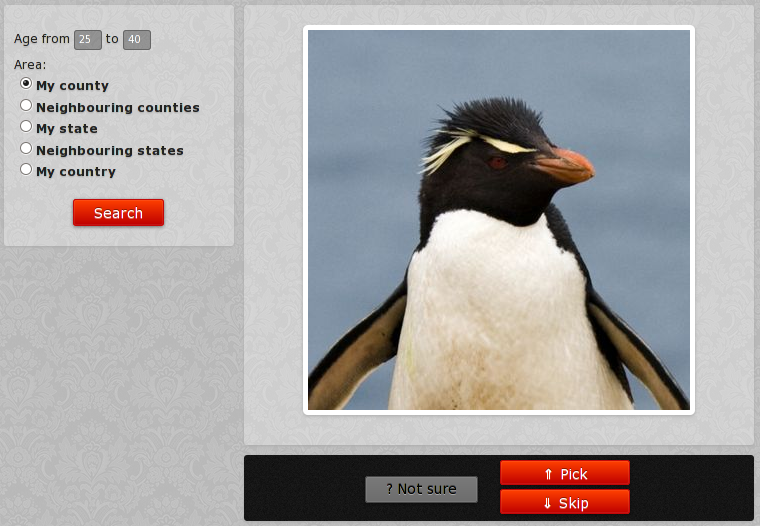
\includegraphics[width=0.8\textwidth]{screen-search.png}
		  \caption{Search and selection screen. (Author of the penguin photo: Samuel Blanc, CC-BY-SA 3.0)}
		  \label{fig:screen-search}
	  \end{figure}
	  
		The form is asynchronously submitted to \texttt{/me/search} using HTTP \texttt{POST}. The parameters are validated on the server side and saved as a \texttt{JSON} string to the \texttt{user:<id> searchDefaults} hash. This is useful, because the client side JavaScript can use it to load the last used serach paramets directly.
		
		An excerpt of the first phase of the search procedure is shown in listing \ref{code:ex-search}. First a union of sets of appropriate years of birth is created. It is saved in a temporary set that automatically expires in 10 seconds. Similarly a set of users is created according to the specified location.
		
		\begin{program}[h]
		\caption{An excerpt of the search procedure --- first phase}
		\label{code:ex-search}
		\inputminted[fontsize=\footnotesize, linenos=false, gobble=6]{javascript}{ex-search.js}
		\end{program}

		These two sets and, two other for gender selection and one with enabled users are then intersected and visited users are substracted, see listing \ref{code:ex-search1}. A maximum of 50 user IDs are returned as a \texttt{JSON} array.
		
		\begin{program}[h]
		\caption{An excerpt of the search procedure --- second phase}
		\label{code:ex-search1}
		\inputminted[fontsize=\footnotesize, linenos=false]{javascript}{ex-search1.js}
		\end{program}
	
		The procedure can be in a simplified way written as this set fomula:
		\[
			\left( \bigcup YOB_i \cap \bigcup GEO_i \cap GENDER \cap ENABLED \right) \setminus SEEN
		\]
		We can see that this relatively simple task is rather complex to implement in Redis. The big upside however is that from testing with a database of 200 000 users, the whole HTTP request takes about 2ms on recent server hardware and all the command used have $O(n)$ or better complexity.
	
		The user can then mark the resulting photos one-by-one, with more results loading automatically. The "Not sure" choice is used when a photo does not correctly depick the person. When such user then changes the photo, he or she is shown once again. 
		
		The user also has the ability to browse through visited photos and change the decision.
		\clearpage
	\subsection{Notifications}
		Every time a user marks someone positively, a check is made to see if the liking is mutual. In that case to the \texttt{user:<ID1,ID2>:match\_q} sorted sets ($z$-value\footnote{$z$ is the value based on which the elements in the set are sorted.} is current time) that act as queues. The $z$-value of the sorted set \texttt{user:zsets:match\_pending} is increased by 1 for both users. Users that have disabled their accounts are no longer notified.
		
		The \texttt{notification.js} script is running as a separate background process. It is used to regularly check for notifications for both matches and chat (more on that in section \ref{section:chat}) and to send appropriate e-mails. It sets up a timer that ensures the match notifications are sent only once a day during the night. It can be gracefully quit by sending the \texttt{SIGQUIT} UNIX signal (in a similar way to the \texttt{worker-email.js} script shown later in listing \ref{code:ex-emailworker}).
		
		The whole purpose of the rather complicated \texttt{matchNotify} function is to make sure as many as possible matches are made, but at most one new per user per day. This is the maximum bipartite matching problem. Efficient algorithms to correctly solve it exist. \cite{Galil1986} However here for the sake of simplicity a naive algorithm is used --- users with the lowest number of pending matches are handeled first, with oldest pending matched taking precedence. It works reasonably well, as the vast majority of matches are one-on-one and even in case of slight congestion, a few days waiting time for the match to be handeled is not a big problem. That said, this is something that could be improved.
		
		When a match is handeled, both users are notified using e-mail and are added to one another's contact lists to be able to engage in chat.
	\subsection{Chat}
		Implementation of the chat screen is shown in figure \ref{fig:screen-chat}.	Available contact are listed on the left side. Those currently online are marked with a red square in the bottom right. If there are unread messages, their count is displayed in the top left. Red border marks currently active chat session.
		
		Message history is displayed in the centre and smooth-scrolls as new messages arrive. Textarea for message input is place below. It automatically grows with the text length. If the box on the right of it is checked, the message is sent when the Return key is pressed, otherwise a new line is created. This allows for both quick chatting without using the mouse and writing of properly formatted messages.
	
		\label{section:chat}
		\begin{figure}[h]
	  \centering
	    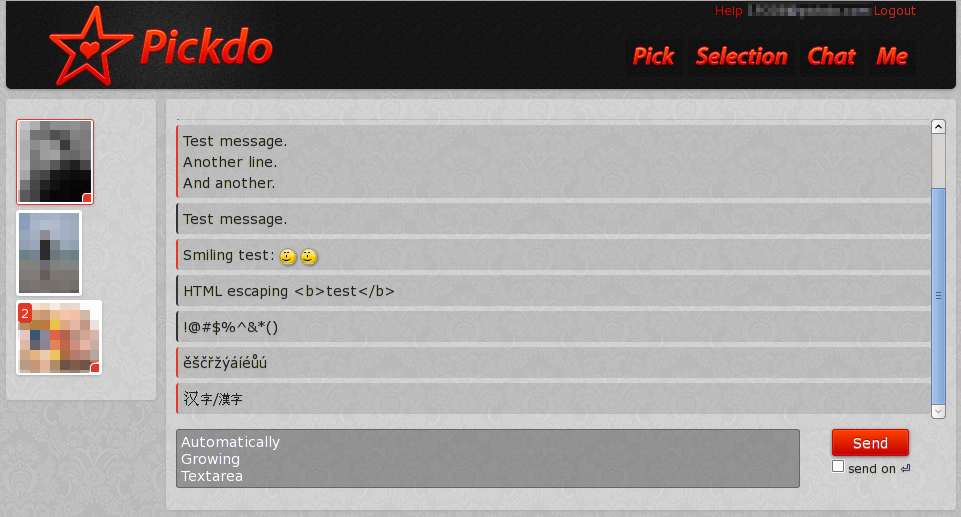
\includegraphics[width=1.0\textwidth]{screen-chat.png}
		  \caption{Chat page}
		  \label{fig:screen-chat}
	  \end{figure}
	  
	  A timer is set on the client side that makes and asynchronous request every 2.3 minutes to \texttt{/me/ping}. The server stores the last ping time in the \texttt{user:zsets:ping} sorted set and returns list a JSON list of contacts that are online, i.e. have sent their ping in the last 2.5 minutes.
	  
	  All messages are asynchronously posted to \texttt{/me/sendmessage}. There it is stored as JSON object to the conversation history. If the number of messages in the history is above 100, the 10 oldest are deleted. Number of unread messages in the \texttt{user:<recipient ID>:unread <sender ID>} hash is increased. Also the \texttt{global:chat\_q} sorted set is updated with current time as the $z$-value for the recipient ID. Lastly the message is published to both sender and recipient \texttt{push:chat:<ID>} Redis subscriber channels.
	  
	  The \texttt{socketio.js} script is running as a separate background \texttt{socket.io} server on port 8080. All connections are authorized using the session cookie. Then it simply listens on the appropriate Redis \texttt{push:chat:<ID>} channels and pushes any new messages to the client. Currently the \texttt{xhr-polling} method is the only one enabled, since WebSocket has been disabled on most web browsers for security reasons and the protocol is going to have to be revised.
	  
	  The \texttt{socket.io} client listens for incoming messages. When a new one is received, it is displayed in the chat history or a visual notification is made. When the message is read, this fact is acknowledged to \texttt{/me/ackmsg/<sender ID>}. There the appropriate unread message count is reset.
	  
	  An e-mail notification about a new message is sent by the \texttt{notification.js} script if all of the following conditions are met (checked every minute):
	  \begin{compactitem}
	  	\item The message is unread and the user has not yet been notified about it.
	    \item The user is offline for a long time --- more than 60 minutes have passed since the last ping.
	    \item More than 3 minutes have passed since the last message addressed to the user.
	  \end{compactitem}
	  This ensures the user is not overwhelmed with notifications.
\section{Implementation in detail}
	\subsection{E-mail sending}
		\label{section:email}
		Whenever the application needs to send an e-mail, it pushes the following JSON object to the \texttt{worker:email:\{p1,p2\}} Redis list, where \texttt{p2} has higher priority that \texttt{p2}.
		\inputminted[fontsize=\footnotesize, linenos=false]{javascript}{ex-emailobj.js}
		
		The \texttt{worker-email.js} background process uses \texttt{async}'s \texttt{whilst} function and Redis's \texttt{BLPOP} command to non-blockingly poll for new e-mails as shown in listing \ref{code:ex-emailworker}. The \texttt{BLPOP} command pops and item from the list if the list is non-empty or waits for a specified amount of seconds for a new item. If it doesn't appear it returns \texttt{null}. The process is safely killable by sending the \texttt{SIGQUIT} UNIX signal.
		
		\begin{program}[h]
		\caption{The e-mail worker}
		\label{code:ex-emailworker}
		\inputminted[fontsize=\footnotesize, linenos=false]{javascript}{ex-emailworker.js}
		\end{program}
		
		The e-mails themselves are sent using the cloud Amazon Simple Email Service (SES -- \url{http://aws.amazon.com/ses/}). It has very favorable pricing at 0.10USD per 1,000 e-mails plus data transfer at approx. 0.10USD per 1GB. Using this service spares the resources of running and administering one's own SMTP server and gives benefits in delivery rates, becouse Amazon checks outgoing e-mails for signs of spam, which gains it a more trusted status among e-mail client's anti-spam  filters.
	\subsection{Security}
		Security of the application is essential for both users and operators. There are many attack vectors hackers could use to compromise them. \cite{paper:dd} Here is a list of those applicable attacks and measures that have been taken to prevent them:
		\begin{itemize}
			\item[\textbf{Parameter tampering}] 
				Because of the nature of HTML/HTTP, it is very simple to send parameters that are not allowed by the client side of the application. Hence, before any request is processed, it is passed through a series of \texttt{connect} filters. The \texttt{limit} fitler built-in to \texttt{express} limts the size of \texttt{POST} parameters to a given amount --- here 100KB. \texttt{GET} parameters are automatically limited to 8KB by Node.js. Moreover lenghts of all fields are then checked by the custom \texttt{paramLength} filter. 
			\item[\textbf{Cross-site scripting}] 
				This attack is possible whenever user content is displayed to other users. In this project is basically happend at two points: the profile photo and chat. The profile photo is always checked to be of the correct format. All chat messages are properly HTML escaped before they are displayed.
			\item[\textbf{SQL-injection}]
				Cannot be applied directly because Redis is a NoSQL data store. All Redis commands have a fixed structure and user content is always passed as binary-safe data and no plain text queries are used, as opposed to SQL. There is one exception: key names with \texttt{id} (such as \texttt{"user:"+id+":email"}) are constructed from user data, but these parameters are always converted to integer before usage. Any such attacks are therefore impossible.
			\item[\textbf{Authorization}] In the best case, all client-server communication should be run through a secure channel, i.e. SSL, TLS, HTTPS. This is however very demanding on the servers or requires a dedicated SSL acceleration hardware, both beign cost prohibitive for now.
			\item[\textbf{Cookie theft}]
				Authorization is cookie-based, so the possibility of this attack indeed exsists. However to minimaze the risk, \texttt{connect} uses cryptographically signed cookies with fingerprints (e.g. client IP address, browser \texttt{User-Agent} header etc.), so the attacker would not only need to steal the cookie, but also to emulate all there paramaters, which is close to impossible.				
		\end{itemize}		
	\subsection{Internationalization}
		Server-side internationalization is facilitated by the \texttt{i18n.js} module, which is a version of the original by Marcus Spiegel extended with this functionality:
		\begin{compactitem}
			\item Option to set a default locale
			\item Get locale from session automatically
			\item Translate messages to a locale specified by parameters independently of the request (the \texttt{l\_\_} function)
		\end{compactitem}
		Messages are stored as a JSON object in files, e.g. \texttt{locale/en.js}.
		
		Because many user actions happen asychronously, client-side internationalization is also present. Messages are again stored as a JSON object (\texttt{locale/en\_client.js}) and are directly inserted in the HTML file in a \texttt{<script>} tag creating the \texttt{t} global variable. There are no parametrized messages on the client side, so this simple approach suffices. Otherwise the server-side \texttt{i18n.js} module could be easily ported to client side, since both employ JavaScript.
	\subsection{Geolocation}
	\label{section:geo}
		All geolocation data used in the application comes from the Yahoo! GeoPlanet project. \cite{website:geoplanet} It provides both a web service, which allows for searching of the database, and the source data tables. Here the \texttt{places} and \texttt{adjacencies} tables are used. Every place in the database has it unique constant ID called WOEID (Where On Earth ID). 
		
		The \texttt{places} table contains all the places available, their names, WOEIDs, types and parents' WOEIDs. The \texttt{adjacencies} table simply contains pairs of WOEIDs of the same level that are geographically adjacent.
		
		The \texttt{geo\_fill.py} Python script is used to fill the geolocation database of the application from the provided GeoPlanet database. Complete structure of the generated database is listed in appendix \ref{appendix:scheme} under the \texttt{geo:} prefix.
	\subsection{Performance tuning}
		Both Node.js and Redis are single-threaded, therefore performance can be significantly improved by runnig multiple instances of them. With Node.js this can be easily achieved by using the \texttt{cluster} module that can manage startup, zero-downtime reloading and stopping of the instances. 
		
		With Redis this is more complicated, because the instances have their own data. Technique called \emph{sharding} can be used to solve this. It spread keys with variable name such as \texttt{user:<ID>:email} across $n$ instances by caclutating \texttt{ID}$\mod{n}$. This is however unpractical here, because set operations are heavily used those and cannot be done when the sets are stored in different instances. So at least the session data is stored in an instance separate from the rest. Redis also features simple master-slave replication that could also be employed.
		
		All client-side JavaScript is combined into one file and minified using \texttt{uglify-js} to improve loading speed. For the same reason Gzip compression is utilized to serve text-based static files.
	\subsection{Graphical design and user experience}
		Attractive graphical design is essential for the success of any web application. The author has tried to do his best in this area. Advanced CSS3 effects such as gradients, text- and box-shadows, opacity and transitions are used as well as JavaScript animations.
		
		Once the user logs in, all operations are done asynchronously. Not only does this reduce server load but also greatly improves user experience and responsivness.
\chapter{Conclusion}

\appendix
\chapter{Structure of the storage}
\label{appendix:scheme}
\texttt{<id>} --- mutable parameter\\
\texttt{*} --- stored as hash
\inputminted[fontsize=\footnotesize]{yaml}{scheme.txt}

% Následují další kapitoly a podkapitoly, popřípadě závěr, dodatky, 
% seznam literatury či použitých obrázků nebo tabulek.

\bibliographystyle{plain}  % bibliografický styl 
\bibliography{bp} % soubor s citovanými
                           % položkami bibliografie 

\end{document}